\setcounter{chapter}{2}
\chapter{Specifikacija programske potpore}

\section{Funkcionalni zahtjevi}

\noindent \textbf{Dionici:}

\begin{enumerate}
	
	\item Kupci 
	\item Ponuditelji
	\begin{enumerate}
		\item Izdavač
		\item Antikvarijat
		\item Preprodavač
	\end{enumerate}	
	\item Administrator		
	\item Razvojni tim
	
\end{enumerate}

\noindent \textbf{Aktori i njihovi funkcionalni zahtjevi:}


\begin{enumerate}
	\item  \underbar{Neregistrirani korisnik (inicijator) može:}
	
	\begin{enumerate}
		
		\item pretraživati ponude knjiga
		\begin{enumerate}
			
			\item  po značajkama knjige (naziv, autori, godina izdanja, izdavač,
			kategorija izdavača (domaći, strani), žanr, ISBN, broj izdanja, stanje očuvanosti,
			tekstni opis, slika korica, oznaka vrste knjige i lista ponuda)
			\item  po nazivu ponuditelja (izlistati sve knjige dotičnog)
			\item na karti (npr. OpenStreetMap) gdje su označene lokacije svih ponuditelja knjiga
			
		\end{enumerate}
		\item  zatražiti od izdavača da kontaktira stranog izdavača oko prijevoda strane knjige na hrvatski jezik
		
		\item vidjeti popis dostupnih ponuda za odabranu knjigu, uključujući naziv ponuditelja, broj dostupnih primjeraka i cijenu knjige kod svakog ponuditelja
		
		
		
	\end{enumerate}
	
	\item  \underbar{Svaki ponuditelj (izdavač, antikvarijat, preprodavač) (inicijator) može:}
	
	\begin{enumerate}
		
		\item ponuditi neograničeni broj naslova knjiga i primjeraka knjiga
		\item uklanjati primjerke već postojeće knjige 
		
	\end{enumerate}
	
	\item \underbar{Izdavač (inicijator) može:}
	
	zatražiti izdavača strane knjige za dozvolu prijevoda knjige sa stranog ili srodnog jezika na hrvatski jezik
	
	\item \underbar{Antikvarijat (inicijator) može:}
	
	nuditi knjige na stranom jeziku, srodnom jeziku ili hrvatskom jeziku
	
	
	\item \underbar{Preprodavač (inicijator) može:}
	
	nuditi sve vrste knjiga, uključujući i one koje nisu na drugačiji način dobavljive na području
	Hrvatske
	
	\item \underbar{Administrator (inicijator) može:}
	\begin{enumerate}
		\item odobriti registracije ponuditelja
		\item upravljati korisničkim računima
		\item riješavati sporove i pratiti komunikaciju između neregistriranih korisnika i ponuditelja
	\end{enumerate}
		
	\item \underbar{Baza podataka (sudionik):}
	
	\begin{enumerate}
		
		\item pohranjuje sve podatke o korisnicima i njihovim ovlastima
		
		\item pohranjuje sve podatke o knjigama kao i zahtjeve za prijevod za svaku knjigu na stranom jeziku
		
	\end{enumerate}
	
\end{enumerate}

\eject 



\subsection{Obrasci uporabe}

\subsubsection{Opis obrazaca uporabe}

\noindent \underbar{\textbf{UC1 - Pregled knjiga na karti}}
\begin{enumerate}
	
	\item \textbf{Glavni sudionik: }Neregistrirani korisnik
	\item  \textbf{Cilj:} Pregledati dostupne knjige uz pomoć karte
	\item  \textbf{Sudionici:} Baza podataka
	\item  \textbf{Preduvjet:} - 
	\item  \textbf{Opis osnovnog tijeka:}
	
	\begin{enumerate}
		
		\item Karta je prikazana prilikom učitavanja aplikacije
		\item Neregistrirani korisnik odabire ponuditelja na karti
		\item Izlistavaju se sve knjige dotičnog ponuditelja
		
	\end{enumerate}

\end{enumerate}


\noindent \underbar{\textbf{UC2 - Registracija}}
\begin{enumerate}
	
	\item \textbf{Glavni sudionik: }Neregistrirani korisnik
	\item  \textbf{Cilj:} Stvoriti korisnički račun za pristup sustavu 
	\item  \textbf{Sudionici:} Baza podataka
	\item  \textbf{Preduvjet:} - 
	\item  \textbf{Opis osnovnog tijeka:}
	
	\begin{enumerate}
		
		\item Korisnik odabire opciju za registraciju
		\item Korisnik unosi potrebne korisničke podatke i bira između 3 navedene vrste ponuditelja
		\item Korisnik prima obavijest o uspješnoj registraciji nakon administratorskog pregleda
		
	\end{enumerate}
	
		
	\item  \textbf{Opis mogućih odstupanja:}
	
	\item[] \begin{enumerate}
		
		\item[2.a] Odabir već zauzetog korisničkog imena i/ili e-maila, unos korisničkog
		podatka u nedozvoljenom formatu ili pružanje neispravnoga e-maila ili odabir adrese koja se ne podudara sa pravilima aplikacije
		\item[] \begin{enumerate}
			
			\item Sustav obavještava korisnika o neuspjelom upisu i vraća ga na stra-
			nicu za registraciju
			\item Korisnik mijenja potrebne podatke te završava unos ili odustaje od registracije
			
		\end{enumerate}
		
	\end{enumerate}
	
\end{enumerate}

\noindent \underbar{\textbf{UC3 - Prijava u sustav}}
\begin{enumerate}
	
	\item \textbf{Glavni sudionik: } Ponuditelj
	\item  \textbf{Cilj:} Autentifikacija korisnika
	\item  \textbf{Sudionici:} Baza podataka
	\item  \textbf{Preduvjet:} Registracija
	\item  \textbf{Opis osnovnog tijeka:}
	
	\begin{enumerate}
		
		\item Unos korisničkog imena i lozinke
		\item Potvrda o ispravnosti unesenih podataka
		\item Pristup funkcijama registriranih korisnika, ovisno o tipu ponuditelja
		
	\end{enumerate}
	
	\item  \textbf{Opis mogućih odstupanja:}
	
	\item[] \begin{enumerate}
		
		\item[2.a] Neispravno korisničko ime/lozinka
		\item[] \begin{enumerate}
			
			\item Sustav obavještava korisnika o neuspjelom upisu i vraća ga na stra-
			nicu za prijavu
			
		\end{enumerate}
		
	\end{enumerate}
	
\end{enumerate}

\noindent \underbar{\textbf{UC4 - Pretraživanje knjiga po značajkama knjige}}
\begin{enumerate}
	
	\item \textbf{Glavni sudionik: } Neregistrirani korisnik
	\item  \textbf{Cilj:} Pronalazak željene knjige
	\item  \textbf{Sudionici:} Baza podataka
	\item  \textbf{Preduvjet:} -
	\item  \textbf{Opis osnovnog tijeka:}
	
	\begin{enumerate}
		
		\item Unos značajki knjige u odgovarajuće polje
		\item Izlistavanje knjiga koje se podudaraju sa tim značajkama
		
	\end{enumerate}
	
	\item  \textbf{Opis mogućih odstupanja:}
	
	\item[] \begin{enumerate}
		
		\item[2.a] Nepodudaranje sa ijednom knjigom u bazi podataka
		\item[] \begin{enumerate}
			
			\item Sustav obavještava korisnika o tome da knjiga ili ne postoji ili nije dostupna
			
		\end{enumerate}
		
	\end{enumerate}
	
\end{enumerate}

\noindent \underbar{\textbf{UC5 - Pretraživanje knjiga po nazivu ponuditelja}}
\begin{enumerate}
	
	\item \textbf{Glavni sudionik: } Neregistrirani korisnik
	\item  \textbf{Cilj:} Izlistavanje knjiga određenog ponuditelja
	\item  \textbf{Sudionici:} Baza podataka
	\item  \textbf{Preduvjet:} -
	\item  \textbf{Opis osnovnog tijeka:}
	
	\begin{enumerate}
		
		\item Unos naziva ponuditelja u odgovarajuće polje
		\item Izlistavanje knjiga koje su na ponuditeljevom popisu
		
	\end{enumerate}
	
	\item  \textbf{Opis mogućih odstupanja:}
	
	\item[] \begin{enumerate}
		
		\item[2.a] Nepodudaranje sa ijednim ponuditeljem u bazi podataka
		\item[] \begin{enumerate}
			
			\item Sustav obavještava korisnika o tome da ponuditelj ili ne postoji ili nema nijednu knjigu na trenutnoj ponudi
			
		\end{enumerate}
		
	\end{enumerate}
	
\end{enumerate}

\noindent \underbar{\textbf{UC6 - Zatražiti izdavača da kontaktira stranog izdavača oko prijevoda strane knjige na hrvatski jezik}}
\begin{enumerate}
	
	\item \textbf{Glavni sudionik: } Neregistrirani korisnik
	\item  \textbf{Cilj:} Zatražiti prijevod strane knjige na hrvatski jezik
	\item  \textbf{Sudionici:} Baza podataka
	\item  \textbf{Preduvjet:} Izdavač postoji i pronađen je kroz search
	\item  \textbf{Opis osnovnog tijeka:}
	
	\begin{enumerate}
	 
		\item Neregistrirani korisnik upiše značajke strane knjige
		\item Sustav obavještava korisnika da je upit poslan
		
	\end{enumerate}
	
\end{enumerate}

\noindent \underbar{\textbf{UC7 - Dodavanje knjige}}
\begin{enumerate}
	
	\item \textbf{Glavni sudionik: } Ponuditelj
	\item  \textbf{Cilj:} Dodati dostupnu knjigu 
	\item  \textbf{Sudionici:} Baza podataka
	\item  \textbf{Preduvjet:} Ponuditelj je prijavljen u sustav
	\item  \textbf{Opis osnovnog tijeka:}
	
	\begin{enumerate}
		
		\item Ponuditelj odabere opciju za dodavanje primjerka knjige
		\item Ponuditelj upisuje sve značajke knjige   
		\item Potvrda o upisu knjige u bazu podataka kao nove knjige ili kao još jedan primjerak već postojeće
		
	\end{enumerate}
	
\end{enumerate}

\noindent \underbar{\textbf{UC8 - Uklanjanje knjige}}
\begin{enumerate}
	
	\item \textbf{Glavni sudionik: } Ponuditelj
	\item  \textbf{Cilj:} Izbrisati primjerak knjige
	\item  \textbf{Sudionici:} Baza podataka
	\item  \textbf{Preduvjet:} Ponuditelj je prijavljen u sustav
	\item  \textbf{Opis osnovnog tijeka:}
	
	\begin{enumerate}
		
		\item Ponuditelj odabere opciju za brisanje primjerka knjige
		\item Ponuditelj upisuje sve značajke knjige 
		\item Potvrda o smanjenju primjeraka knjige 
		
	\end{enumerate}
	
	\item  \textbf{Opis mogućih odstupanja:}
	
	\item[] \begin{enumerate}
		
		\item[2.a] Ponuditelj nije niti nudio knjigu ili je već na 0 primjeraka 
		\item[] \begin{enumerate}
			
			\item Sustav obavještava ponuditelja o nemogućnosti uklanjanja primjerka određene knjige
			
		\end{enumerate}
		
	\end{enumerate}
	
\end{enumerate}

\noindent \underbar{\textbf{UC9 - Uređivanje knjige}}
\begin{enumerate}
	
	\item \textbf{Glavni sudionik: } Ponuditelj
	\item  \textbf{Cilj:} Urediti knjigu
	\item  \textbf{Sudionici:} Baza podataka
	\item  \textbf{Preduvjet:} Ponuditelj je prijavljen u sustav
	\item  \textbf{Opis osnovnog tijeka:}
	
	\begin{enumerate}
		
		\item Ponuditelj odabere opciju za uređivanje knjige
		\item Ponuditelj upisuje promjene značajke knjige 
		\item Ponuditelj sprema promjene
		\item Sustav potvrđuje promjene
		
	\end{enumerate}
	
	\item  \textbf{Opis mogućih odstupanja:}
	
	\item[] \begin{enumerate}
		
		\item[2.a] Ponuditelj nije niti nudio knjigu ili je već na 0 primjeraka 
		\item[] \begin{enumerate}
			
			\item Sustav obavještava ponuditelja o nemogućnosti uklanjanja primjerka određene knjige
			
		\end{enumerate}
		
	\end{enumerate}
	
\end{enumerate}

\noindent \underbar{\textbf{UC10 - Neregistrirani korisnik vidi podatke za odabranu knjigu}}
\begin{enumerate}
	
	\item \textbf{Glavni sudionik: } Ponuditelj
	\item  \textbf{Cilj:} 
	\item  \textbf{Sudionici:} Baza podataka
	\item  \textbf{Preduvjet:} Knjiga postoji u bazi podataka
	\item  \textbf{Opis osnovnog tijeka:}
	
	\begin{enumerate}
		
		\item Neregistrirani korisnik klikne na knjigu 
		\item Ispisuje se popis dostupnih ponuda za odabranu knjigu, uključujući naziv ponuditelja, broj dostupnih primjeraka i cijenu knjige kod svakog ponuditelja.
		\item Potvrda o smanjenju primjeraka knjige 
		
	\end{enumerate}
	
	\item  \textbf{Opis mogućih odstupanja:}
	
	\item[] \begin{enumerate}
		
		\item[2.a] Ponuditelj nije niti nudio knjigu ili je već na 0 primjeraka 
		\item[] \begin{enumerate}
			
			\item Sustav obavještava ponuditelja o nemogućnosti uklanjanja primjerka određene knjige
			
		\end{enumerate}
		
	\end{enumerate}
	
\end{enumerate}

\subsubsection{Dijagrami obrazaca uporabe}

	\begin{figure}[H]
	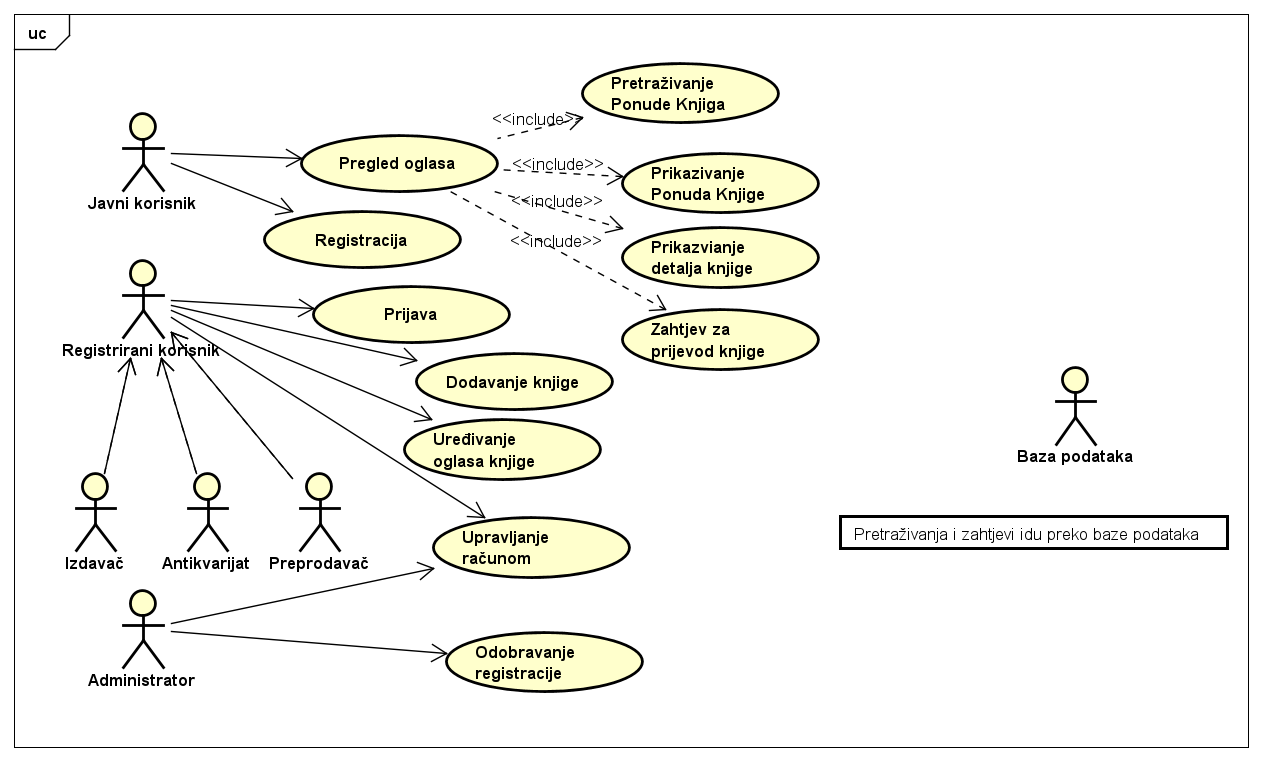
\includegraphics[scale=0.5]{slike/dijagramObrascaUporabe.png} %veličina slike u odnosu na originalnu datoteku i pozicija slike
	\centering
	\caption{Dijagram obrasca uporabe}
	\label{fig:Dijagram obrasca uporabe}
	\end{figure}
	
\eject	

\subsection{Sekvencijski dijagrami}

	\textbf{Obrazac uporabe UC1 - Pretraživanje knjige na karti}
	
	Neregistrirani korisnik šalje zahtjev za ulazak u aplikaciju koja učitava mapu. Neregistrirani korisnik šalje zahtjev za podacima o ponuditelju na kojeg klikne, poslužitelj iz baze podataka dohvaća sve knjige tog ponuditelja te ih vraća ponuditelju.

	\begin{figure}[H]
	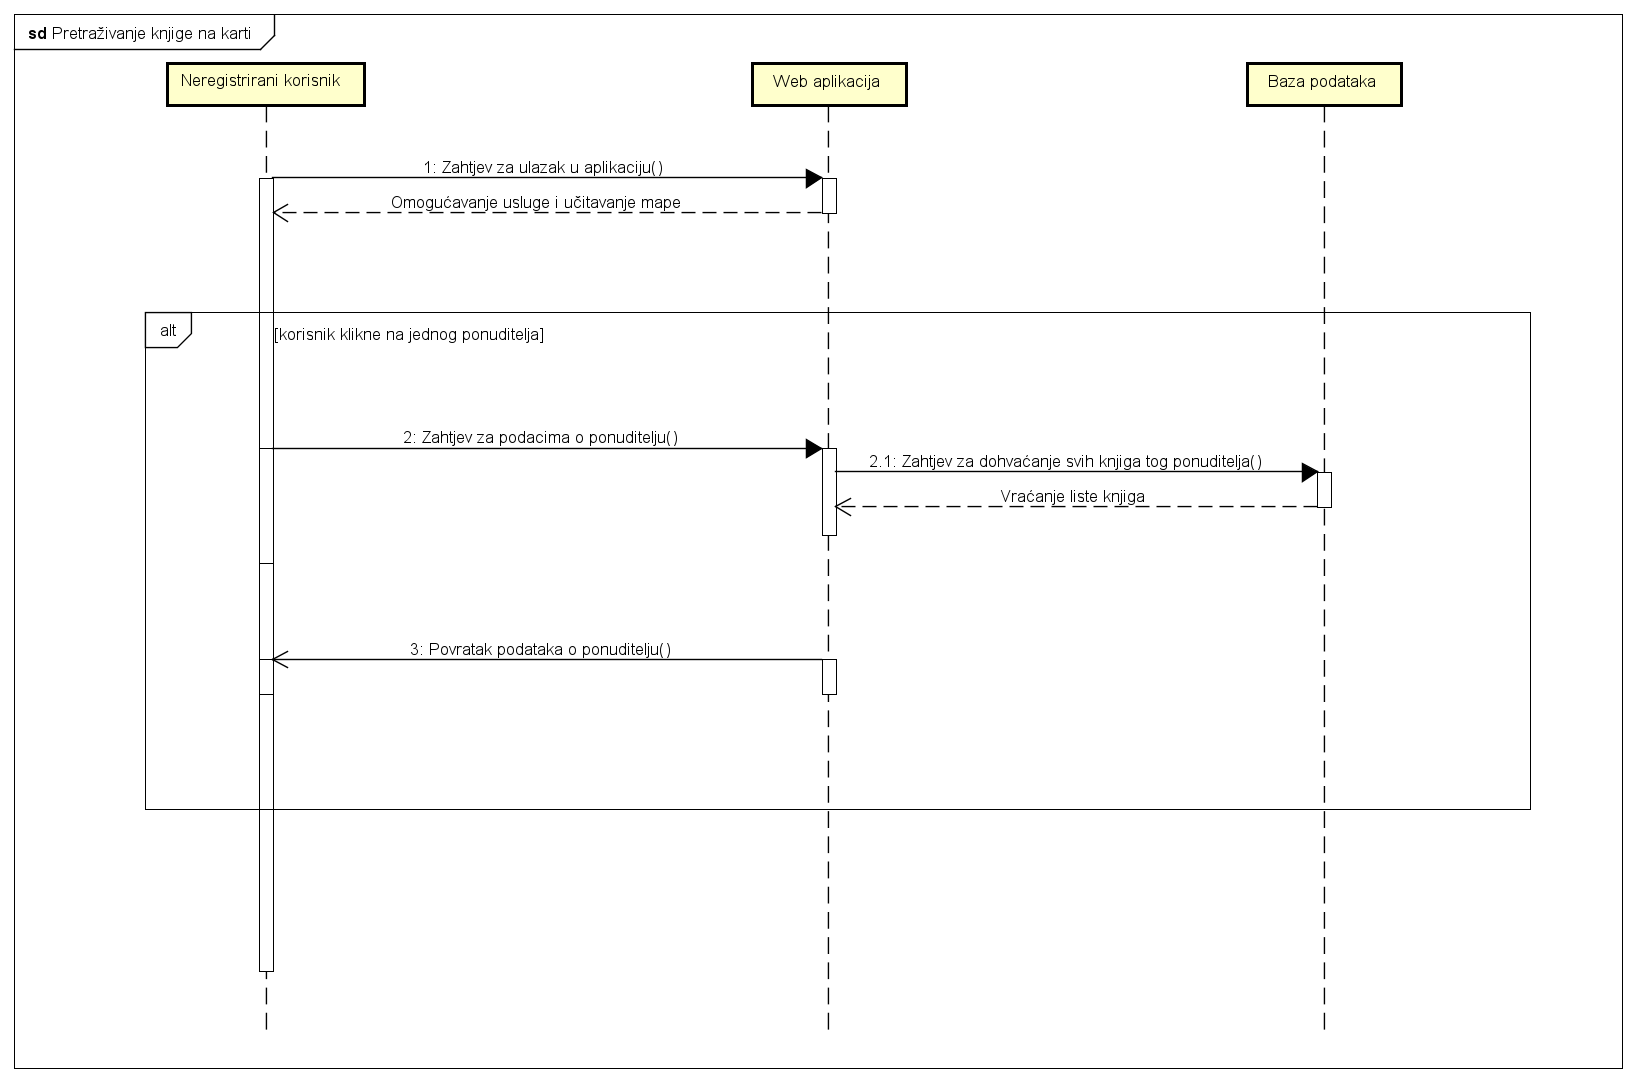
\includegraphics[scale=0.4]{slike/sekvencijskiDijagramPretrazivanjeKnjigeNaKarti.png} %veličina slike u odnosu na originalnu datoteku i pozicija slike
	\centering
	\caption{Sekvencijski dijagram za UC1}
	\label{fig:Sekvencijski dijagam za UC1}
	\end{figure}

\eject	

\textbf{Obrazac uporabe UC2-3 - Registracija i prijava u sustav}

Neregistrirani korisnik šalje zahtjev za registracijom u aplikaciju. Poslužitelj vraća formu za registraciju. Neregistrirani korisnik upisuje podatke, poslužitelj šalje podatke na provjeru pomoću baze podataka. Ako su podaci neispravni, ponavlja se postupak upisa podataka, ako nisu, poslužitelj šalje poruku o ispravnosti. Ako se registrirani korisnik prijavljuje, sve je isto, samo nakon provjere i ako su podaci točni, omogućuje ulaz u sustav registriranih korisnika.

\begin{figure}[H]
	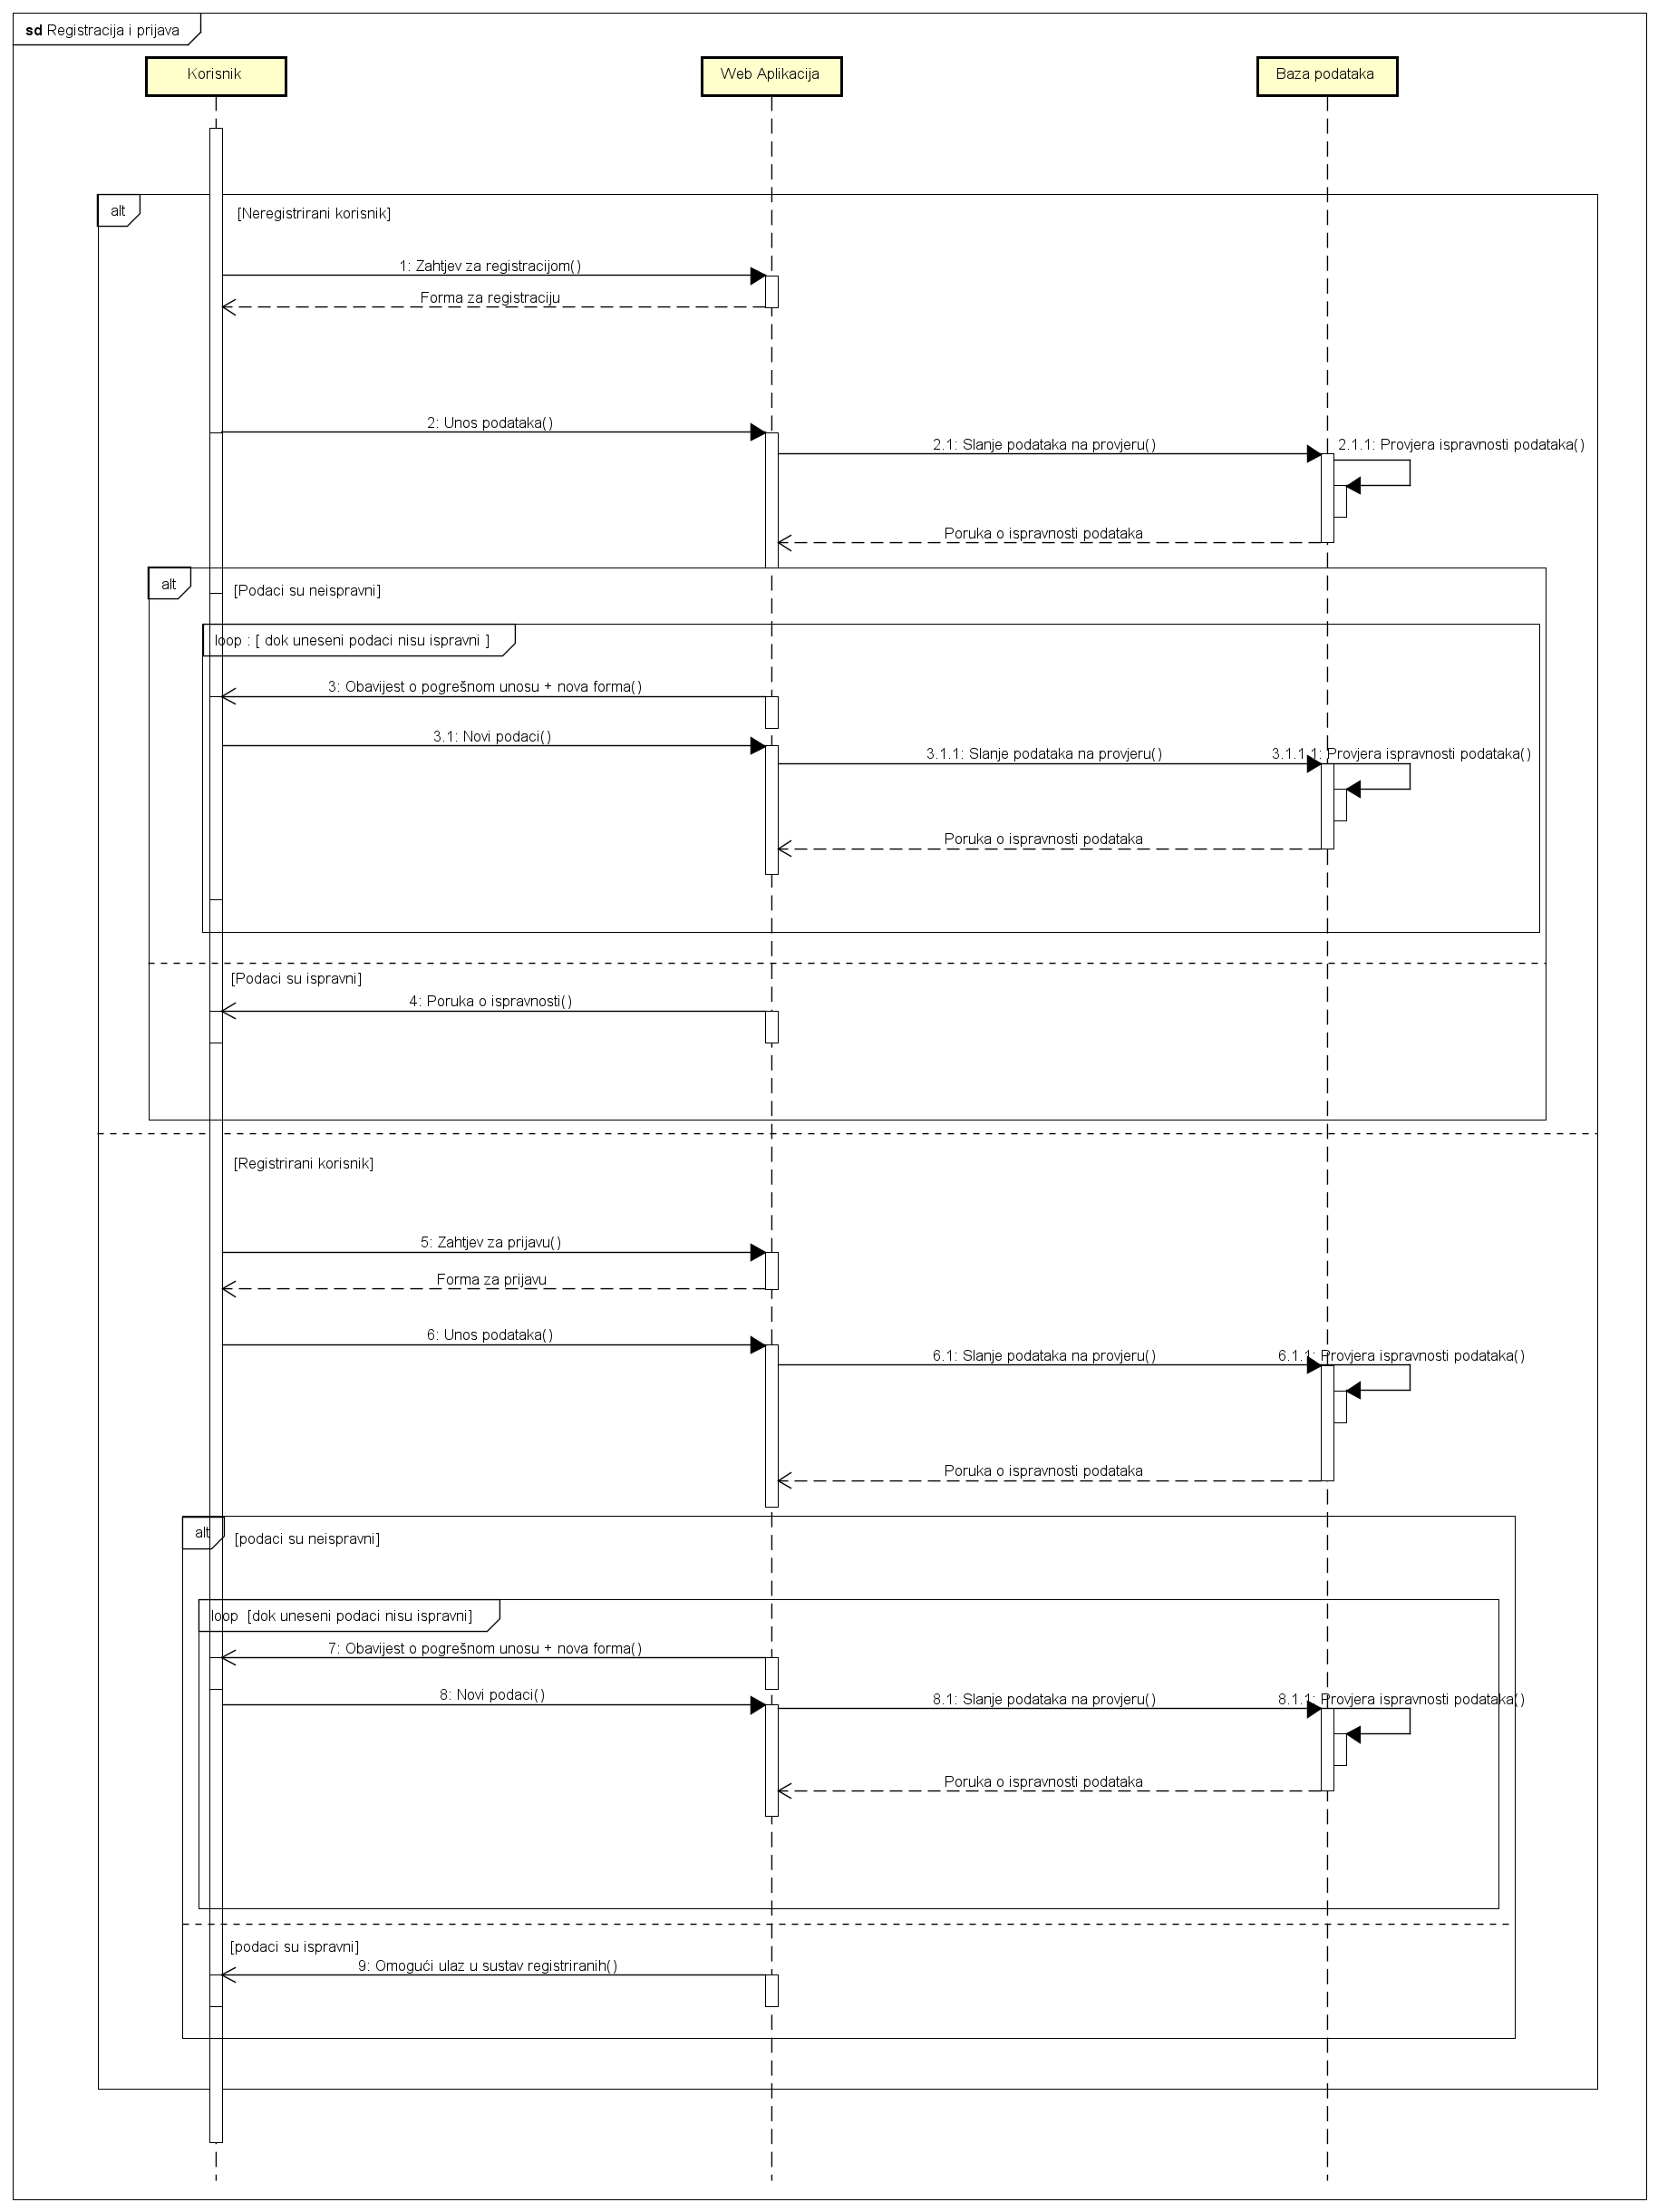
\includegraphics[scale=0.3]{slike/registracijaIPrijava.png} %veličina slike u odnosu na originalnu datoteku i pozicija slike
	\centering
	\caption{Sekvencijski dijagram za UC2-3}
	\label{fig:Sekvencijski dijagam za UC2-3}
\end{figure}

\eject	

\textbf{Obrazac uporabe UC4-5 - Pretraživanje knjige po značajkama knjige i nazivu ponuditelja}

Neregistrirani korisnik šalje zahtjev za pretraživanjem po značajkama, poslužitelj mu vraća formu za unos. Provjeravaju se uneseni podaci te ako nisu ispravni, daje se nova forma za ispunjavanje, a ako jesu, vraćaju se knjige sa tim značajkama. Ista stvar se događa sa pretraživanjem po nazivu ponuditelja, samo se ovdje vraćaju knjige na ponuditeljevom popisu. 

\begin{figure}[H]
	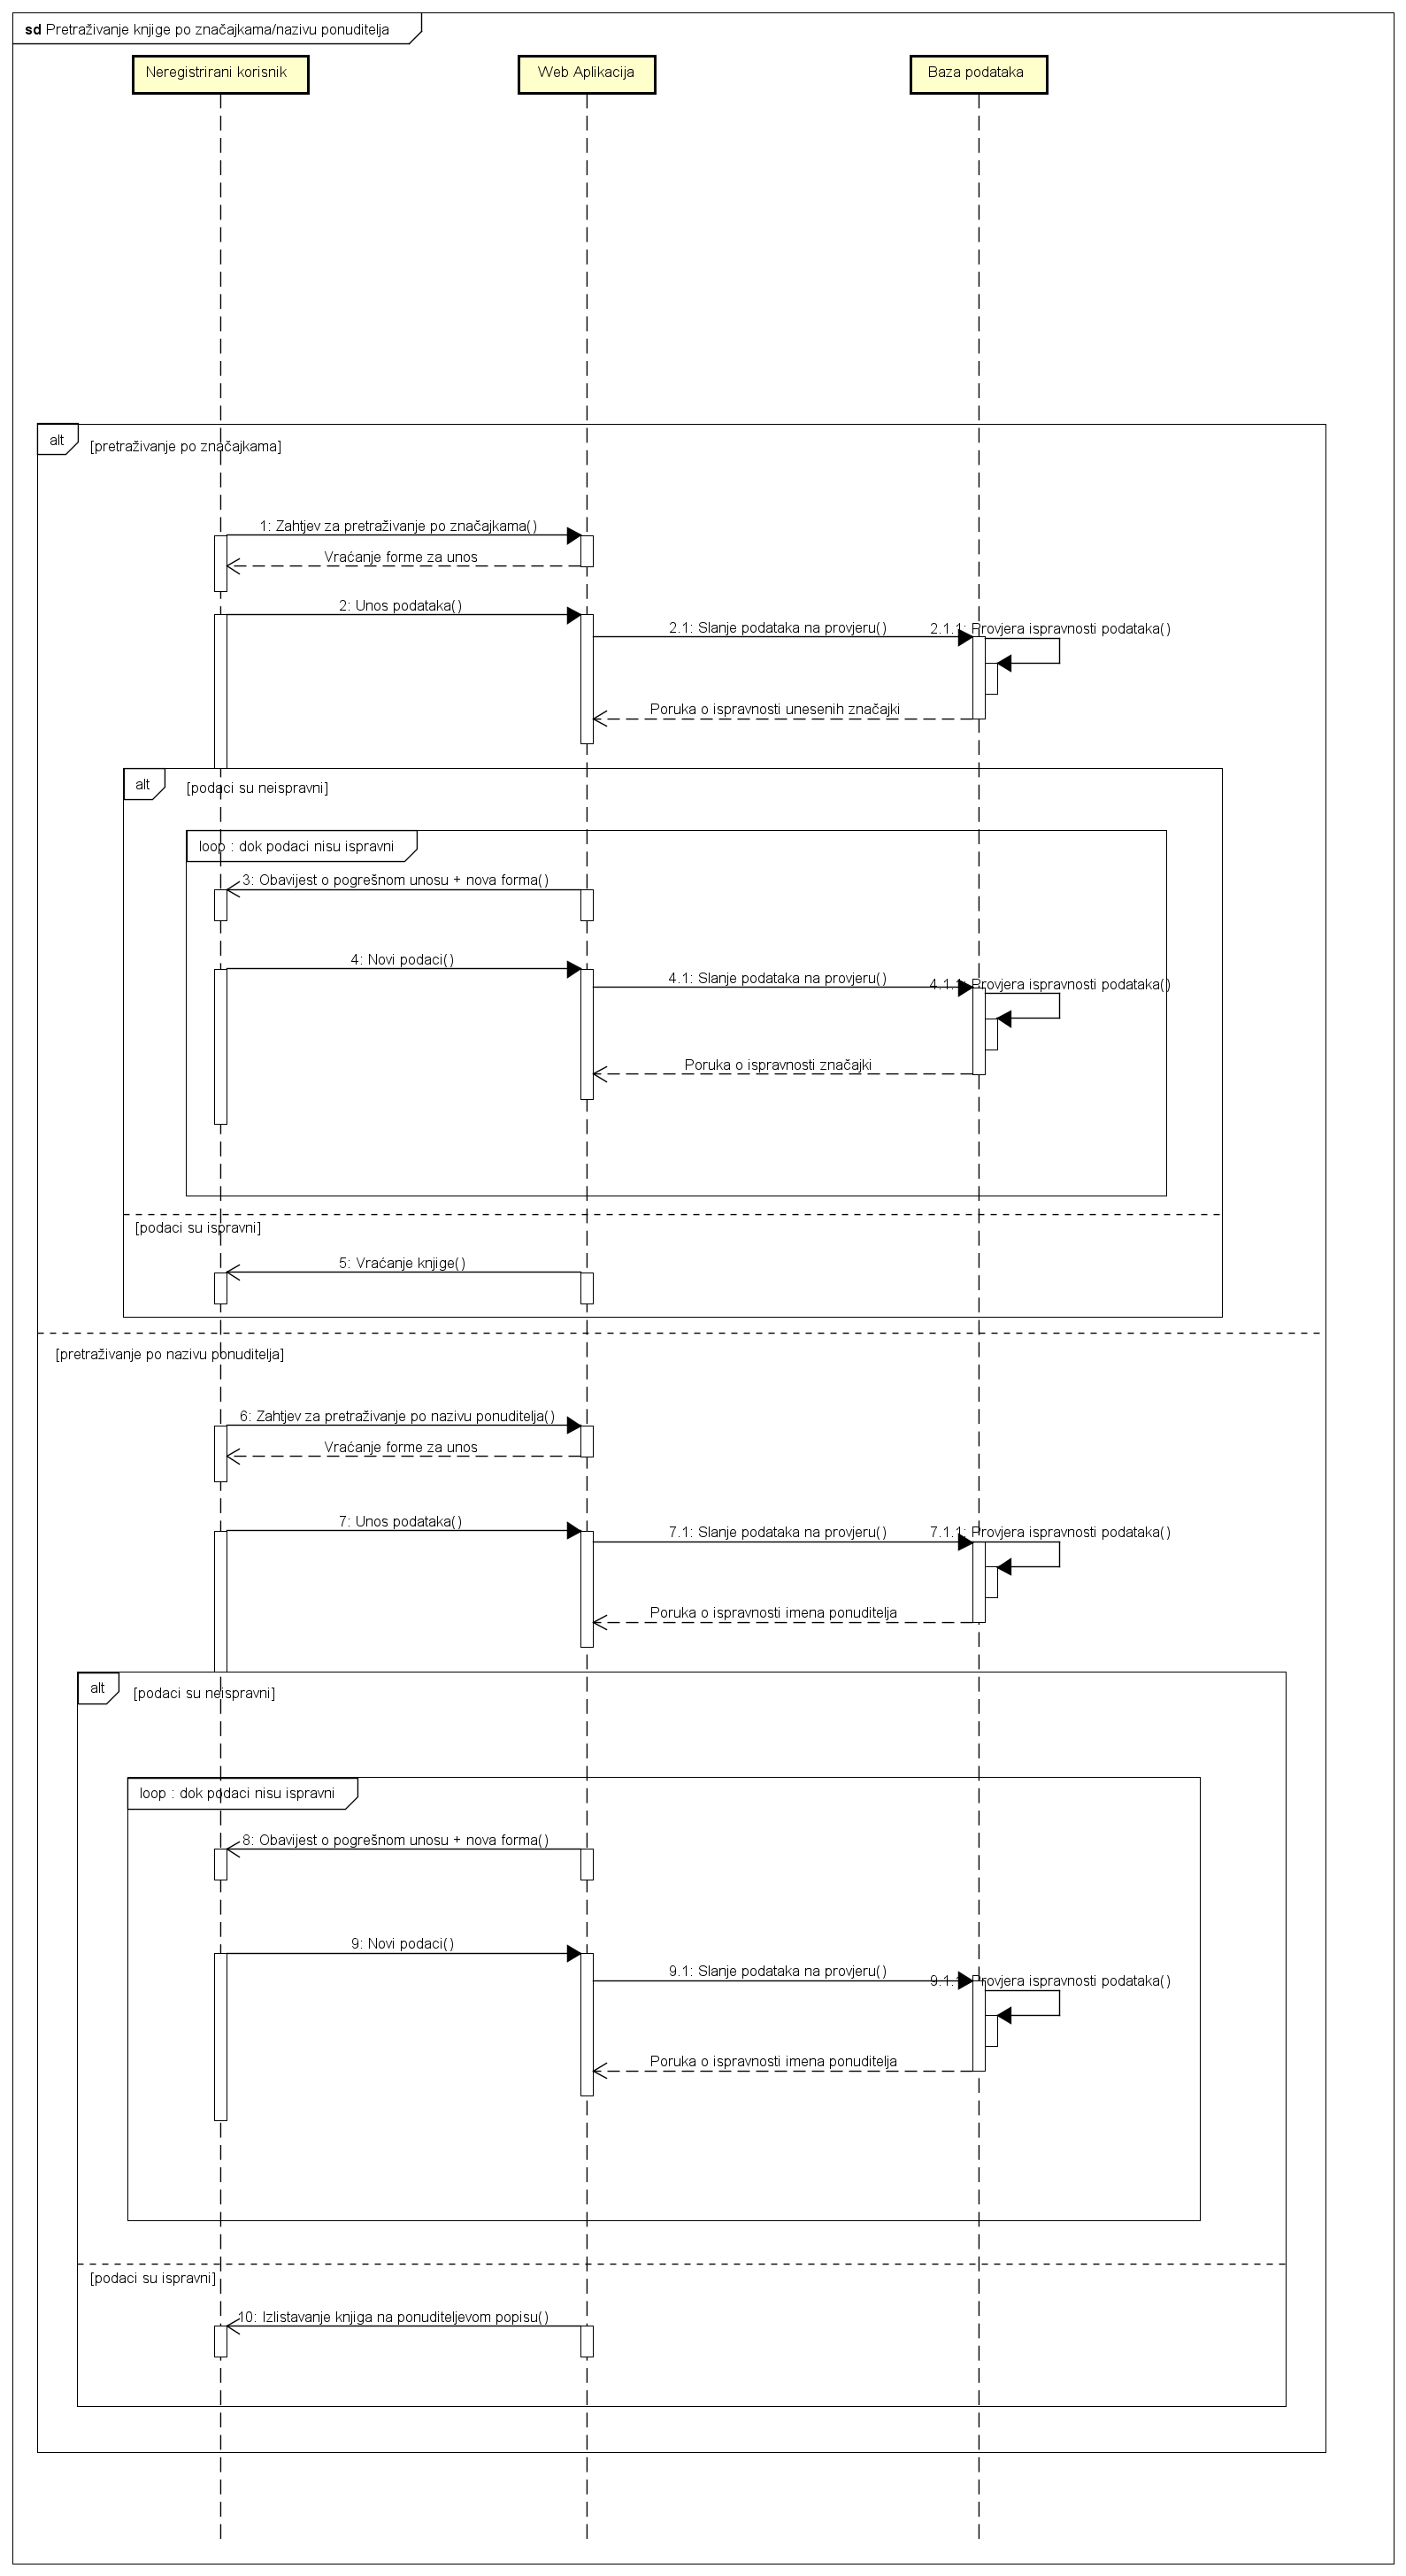
\includegraphics[scale=0.3]{slike/sekvencijskiDijagramPretrazivanjeKnjigePoZnacajkama.png} %veličina slike u odnosu na originalnu datoteku i pozicija slike
	\centering
	\caption{Sekvencijski dijagram za UC4-5}
	\label{fig:Sekvencijski dijagam za UC4-5}
\end{figure}

\eject	

\section{Ostali zahtjevi}
\begin{itemize}
	\item Sustav treba podržavati rad više korisnika u stvarnom vremenu
	\item Ponuditelj može dodati bilo koju knjigu za koju želi da bude ponuđena u aplikaciji, a drugim kanalima može nuditi neke druge knjige
	\item Komunikacija neregistriranih korisnika (onih koji traže neku knjigu) i ponuditelja ne odvija se kroz aplikaciju, već za to služe drugi kanali komunikacije (npr. e-pošta, telefon)
	\item Korisničko sučelje i sustav moraju podržavati hrvatsku abecedu (dijakritičke znakove) pri unosu i prikazu tekstualnog sadržaja
	\item Aplikacija treba biti izvedena kao web aplikacija prilagođena (engl. Responsive) mobilnom uređaju ili tabletu
	\item Registrirani korisnici trebaju joj pristupati uz pomoć korisničkog imena i lozinke
	\item Nadogradnja sustava ne smije narušavati postojeće funkcionalnosti sustava
\end{itemize}
